
\chapter[Domaine métier]{Domaine métier}
Dans le restaurant Crazy Wolf et dans la restauration en général, les employés sont susceptibles de ne pas travailler tous les jours ou de ne pas travailler toute la journée mais seulement certains "services".

Un service est une tranche horaire qui correspond aux heures pendant lesquelles le restaurant offre un service de restauration. Dans le cas concret du Crazy Wolf, il y a deux services: midi et soir. Qui englobent les heures de travail de 9h00 à 15h00 et de 17h00 à 23h00 respectivement. Dans ces tranches horaires sont incluses les heures nécessaires à la disposition du restaurant et d'autres préparations nécessaires avant l'arrivée de clients.

De plus, dans la restauration et surtout en ce qui concerne les serveurs, il est commun d'y trouver trois types d'acteurs avec différents statuts: 
\smallskip
\begin{itemize}
    \item serveur$\cdot$euses
    \item manager 
    \item patrons
\end{itemize}
\smallskip
La gestion, visualisation et organisation des services parmi ces trois acteurs est un élément vital pour un restaurant.

\section[Analyse]{Analyse}
D'après mon observation, la planification de l'horaire de travail des serveurs à un moment donné n'est pas invariante par rapport au temps. En d'autres termes, entre le moment où l'attribution de services aux serveurs est faite et le moment où un serveur y travaille effectivement il peut y avoir de grandes variations. J'ai constaté essentiellement trois facteurs susceptibles de perturber la planification initial:
\smallskip
\begin{itemize}
    \item le désistement d'un$\cdot$e serveur$\cdot$euses
    \item les échanges
    \item la demande de renfort de la part du manager ou d'un patron.
\end{itemize}
\smallskip
Le premier peut être dû à diverses raisons: maladie, imprévu... De plus comme dans le Crazy Wolf, la majorité des serveur$\cdot$euses sont étudiant$\cdot$es les révisions et examens sont fréquemment cause de désistement.

Le deuxième est le fruit d'un mutuel accord entre deux serveurs pour échanger leurs services.

Le troisième est le fruit de l'analyse d’affluence  des clients de la manager en accord avec les patrons. En effet, s'ils constatent que subitement l'afluence des clients augmente le jeudi soir et qu'il y a de fortes chances pour que ce soit aussi le cas le vendredi soir, il sera nécessaire de demander un ou des serveurs supplémentaires. 

Les raisons de cette affluence augmentée peuvent être très diverses. Les conditions météo par exemple. Plus de gens vont au Crazy Wolf quand il pleut, ou en hiver. Ou encore des manifestations comme carnaval ou le marathon.

Dans le jargon propre au Crazy Wolf, ces serveurs supplémentaires sont appelés "doubleurs".

Ainsi, la gestion des horaires est dynamique et non statique.
\newpage
\section[Problématique]{Définition de la problématique}
Actuellement, le Crazy Wolf utilise un groupe, contenant tout le personnel, d'une messagerie instantanée pour communiquer. Dans ce groupe sont traités toute sorte d'aspects. Depuis des félicitations d'anniversaires, jusqu'à l'envoi des horaires mensuels sous forme PDF en passant par des discutions d'échanges, de remplacements, de renforts ou encore sur des discutions relatives aux normes sanitaires dues à la pandémie du COVID-19. 

Ainsi, lorsque la manager demande un renfort pour dans deux semaines et que personne ne se porte volontaire immédiatement, il y a de grandes chances que le message soit répété plusieurs fois.

Il est donc nécessaire de disposer d'une plateforme dynamique, standardisée, centralisée et intuitive dédiée exclusivement à la gestion des horaires. 

Cette plateforme doit être accessible en tout temps depuis internet. Une application fonctionnant sur les deux principaux systèmes d'exploitation mobiles répond bien à ce besoin.

En somme, cette application doit fournir les fonctionnalités suivantes:

\subsection*{Login}
L'application doit permettre aux utilisateurs de s'authentifier pour accéder à l'ensemble des fonctionnalités.

\begin{figure}[!h]
    \begin{center}
        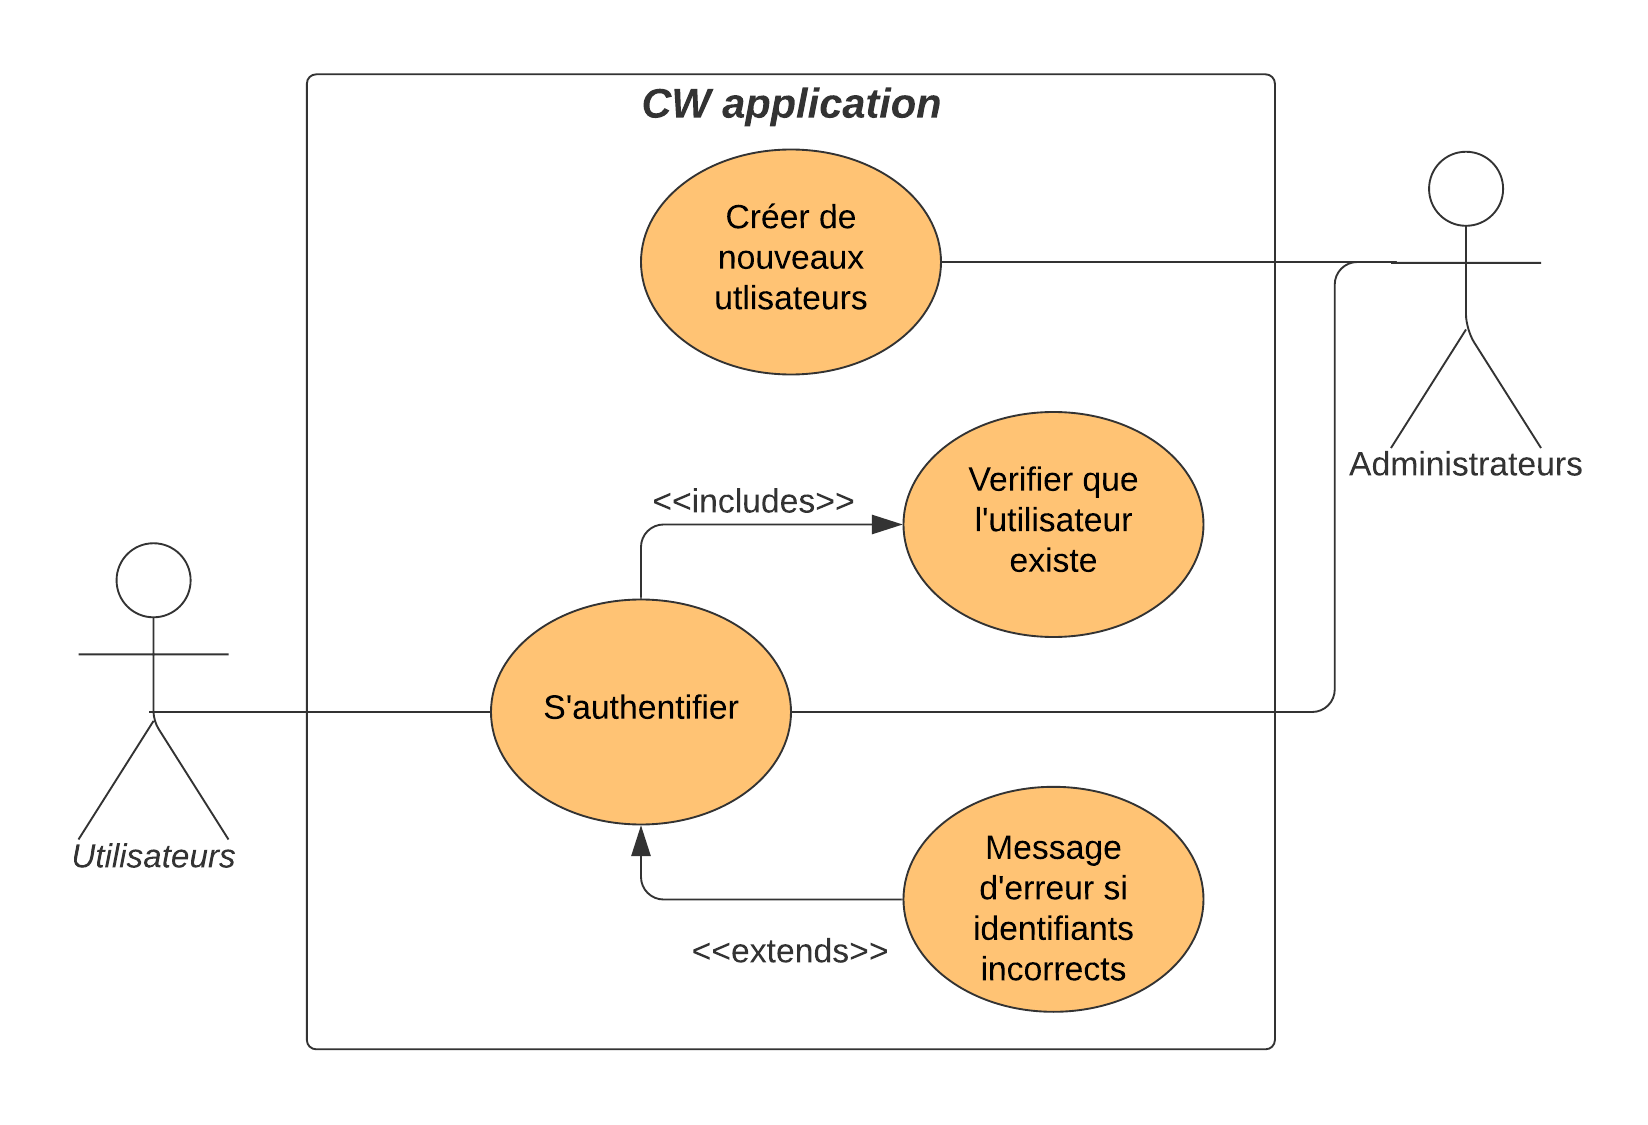
\includegraphics[width= 0.8\textwidth]{uses cases/logginUC.png}
    \end{center}
    \caption{use case: login}
\end{figure}

Pour que l'authentification soit validée, l'utilisateur doit posséder des identifiants qu'un administrateur à créer précédemment. Attention, administrateur doit aussi s'authentifier pour pouvoir créer de nouveaux utilisateurs.

De plus, les utilisateurs doivent être informés si leur saisie est incorrecte.

\subsection*{Visualiser les services}
L'application doit permettre à tous les utilisateurs de consulter rapidement et facilement les services dans lesquels ils travaillent. De plus, ils doivent également pouvoir voir les services dans lesquels les autres utilisateurs travaillent. En effet, il n'y a là aucune information confidentielle.

\begin{figure}[!h]
    \begin{center}
        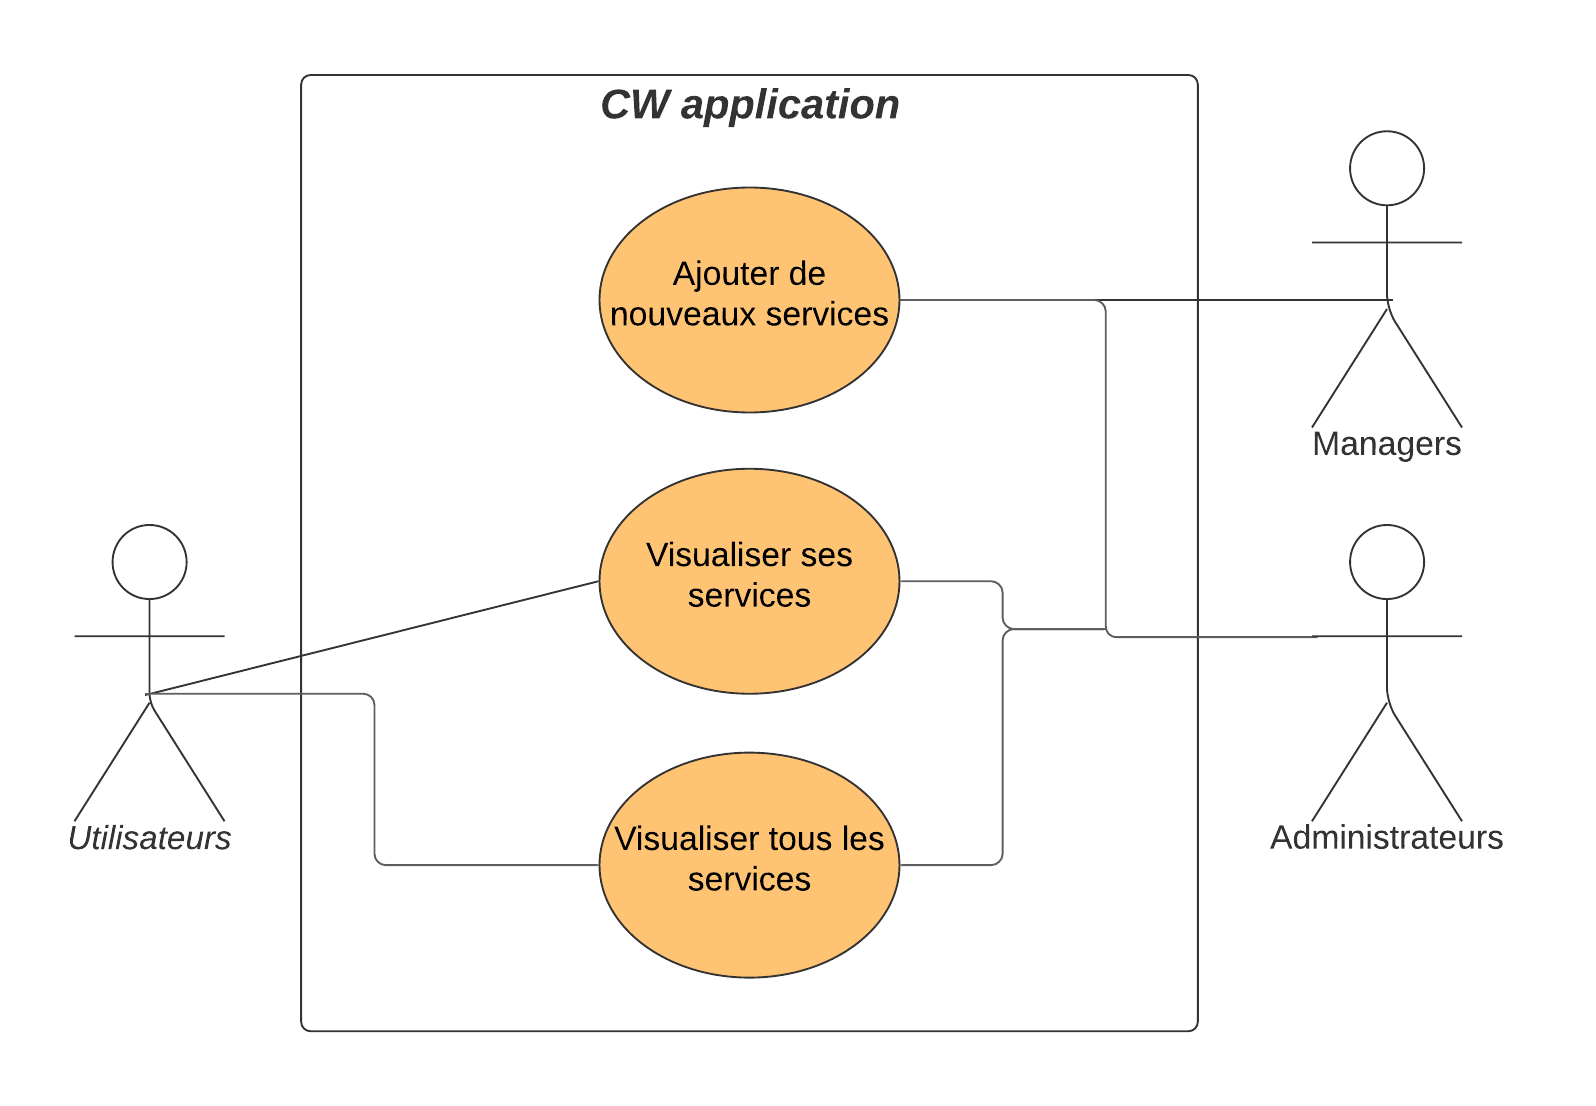
\includegraphics[width= 0.8\textwidth]{uses cases/visualiser services.png}
    \end{center}
    \caption{use case: visualisation des services}
\end{figure}

Afin de pouvoir visualiser des services, il est nécessaire que préalablement, un manager ou un administrateur en ait ajouté dans le système. De plus, le niveau de permission n'exclut pas la possibilité qu'un manager ou administrateur aient des services dans lesquels ils travaillent. Ainsi, ils doivent également pouvoir les visualiser.

\newpage

\subsection*{Mise en bourse}

La mise en bourse d'un service est la fonctionnalité principale de l'application. L'application doit permettre à un$\cdot$e serveur$\cdot$euse de pouvoir mettre un service, où il ou elle ne peut pas travailler, en bourse afin que d'autres utilisateurs de l'application puissent le ou la remplacer.
\begin{figure}[!h]
    \begin{center}
        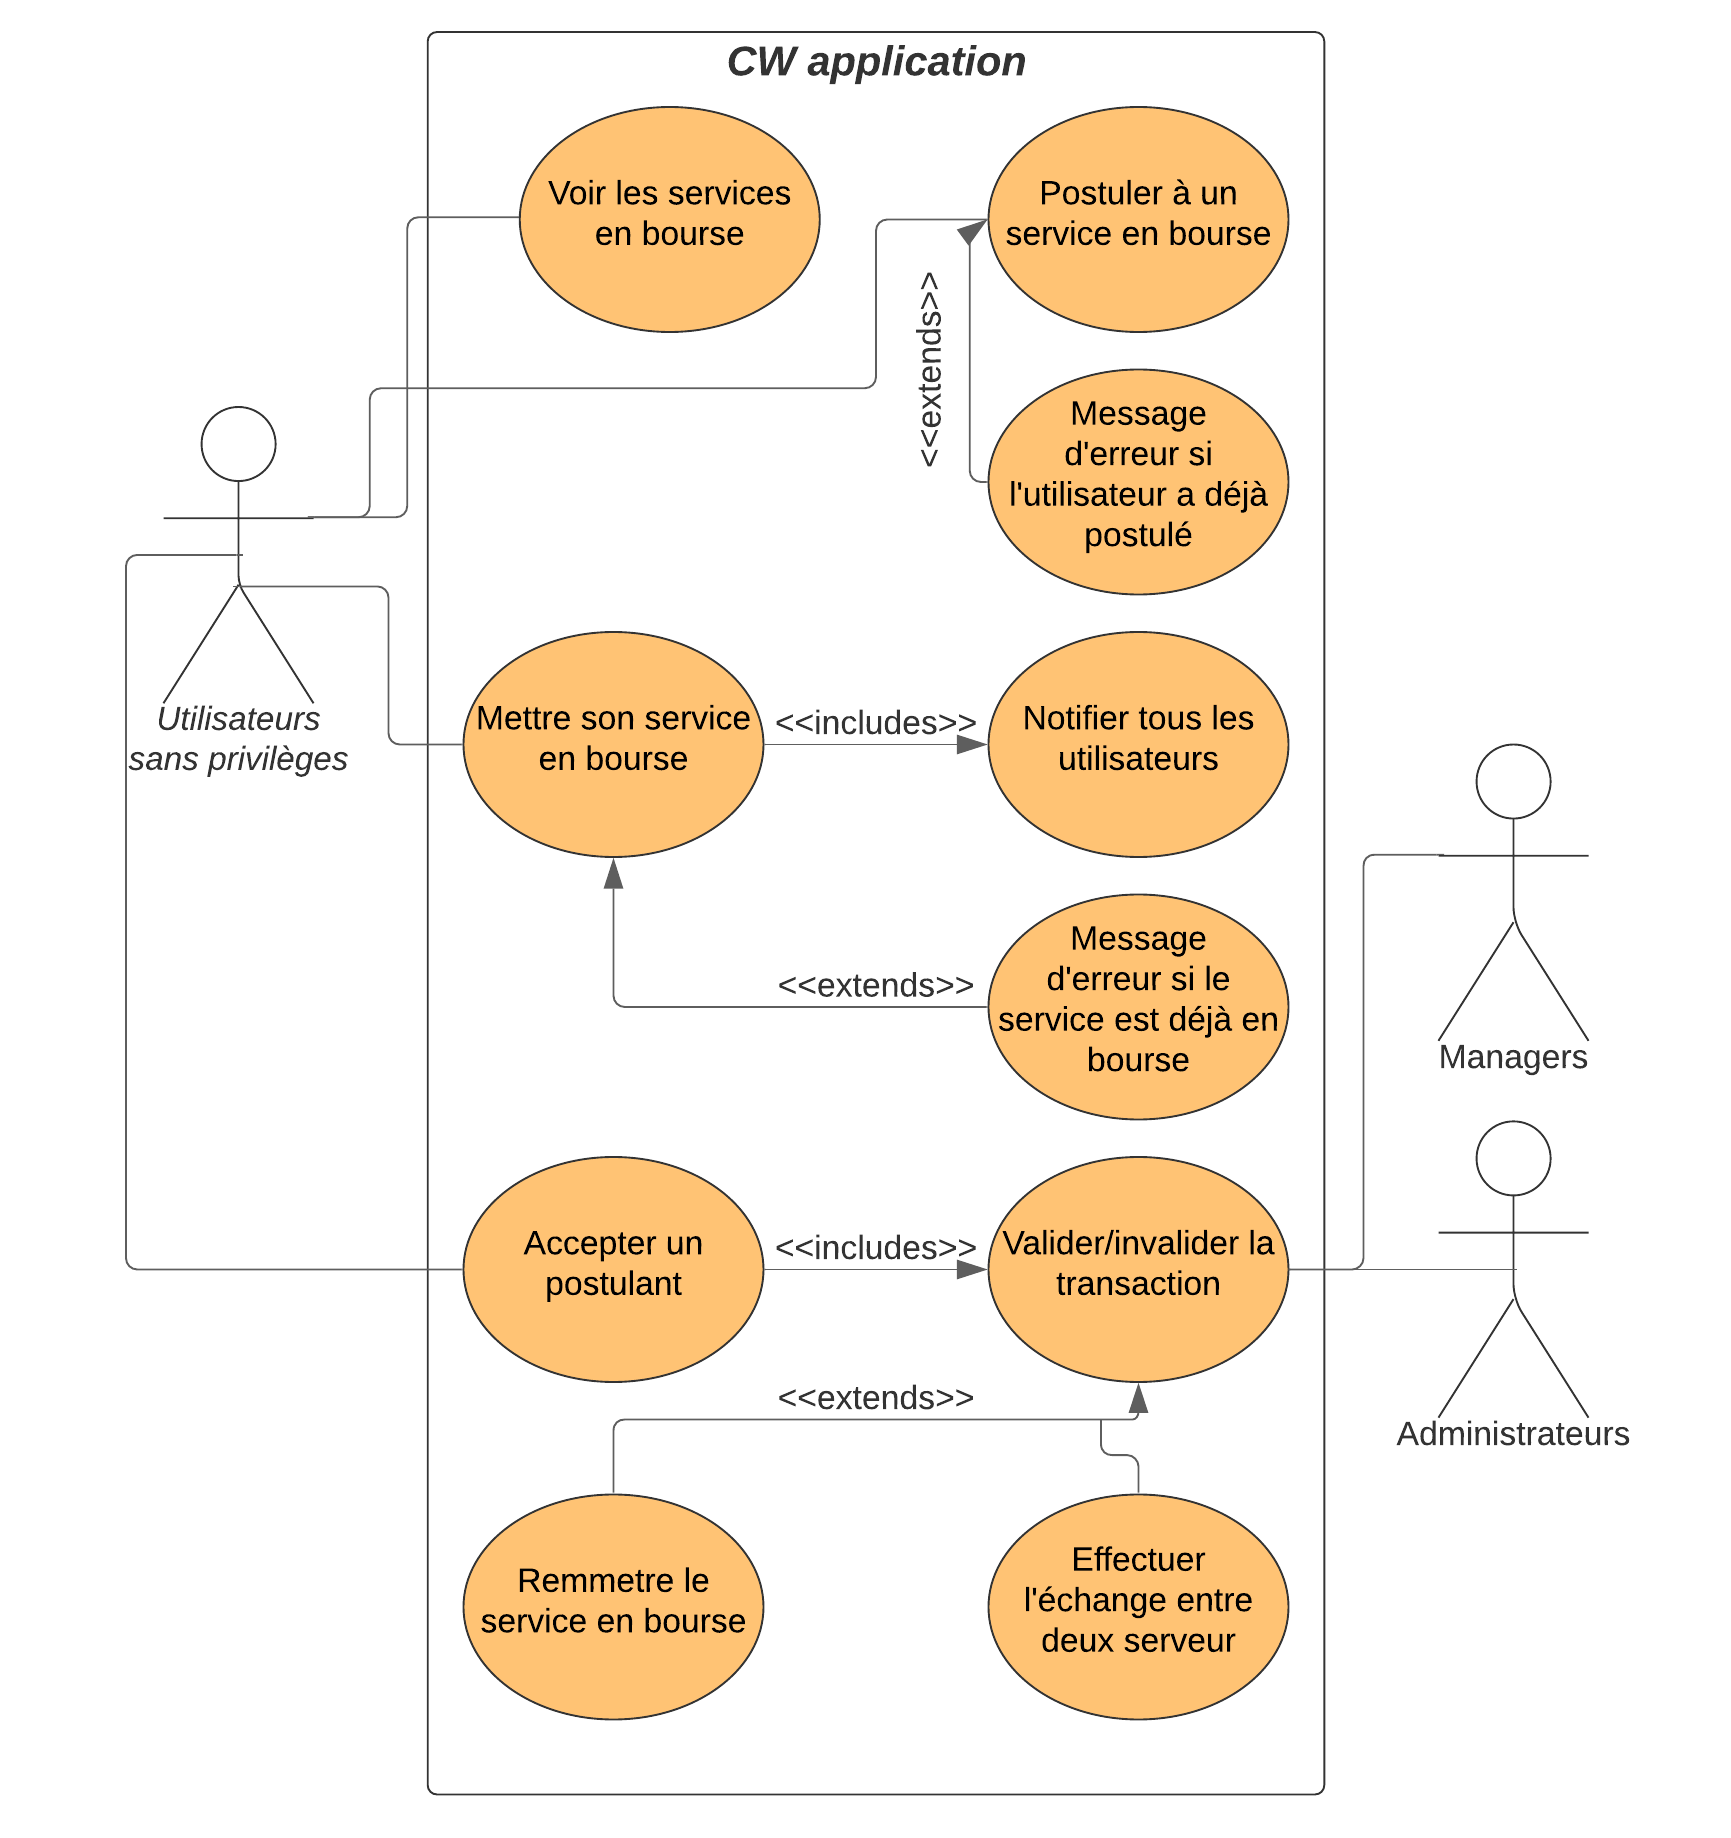
\includegraphics[width= 0.8\textwidth]{uses cases/BourseUC.png}
    \end{center}
    \caption{use case: mise en bourse des services}
\end{figure}

Dans un premier temps, tout utilisateur (normal, manager ou admin) doit pouvoir visualiser les services en bourse.
De plus, tout utilisateur doit pouvoir mettre son et uniquement son service en bourse. Ce qui engendre une notification à l'ensemble des utilisateurs de la disponibilité d'un nouveau service. 

Tout utilisateur doit pouvoir postuler à un service. Cela même si le postulant et celui l'ayant mis en bourse sont la même personne.

Seul l'utilisateur, quel qu'il soit, ayant mis le service en bourse, peut accepter un postulant. Ceci fait, seul un manager ou un administrateur doit valider ou invalider la transaction. Si l'utilisateur ayant mis le service en bourse a des privilèges il peut s'auto-valider la transaction.

Afin de simplifier le diagramme, les restrictions d'un utilisateur normal ont été mise en exergue.

\subsection*{Demande de renfort}

Pouvoir demander du renfort - des serveurs au doublage ou encore des doubleur - est la deuxième fonctionnalité \textit{must be}. 
\begin{figure}[!h]
    \begin{center}
        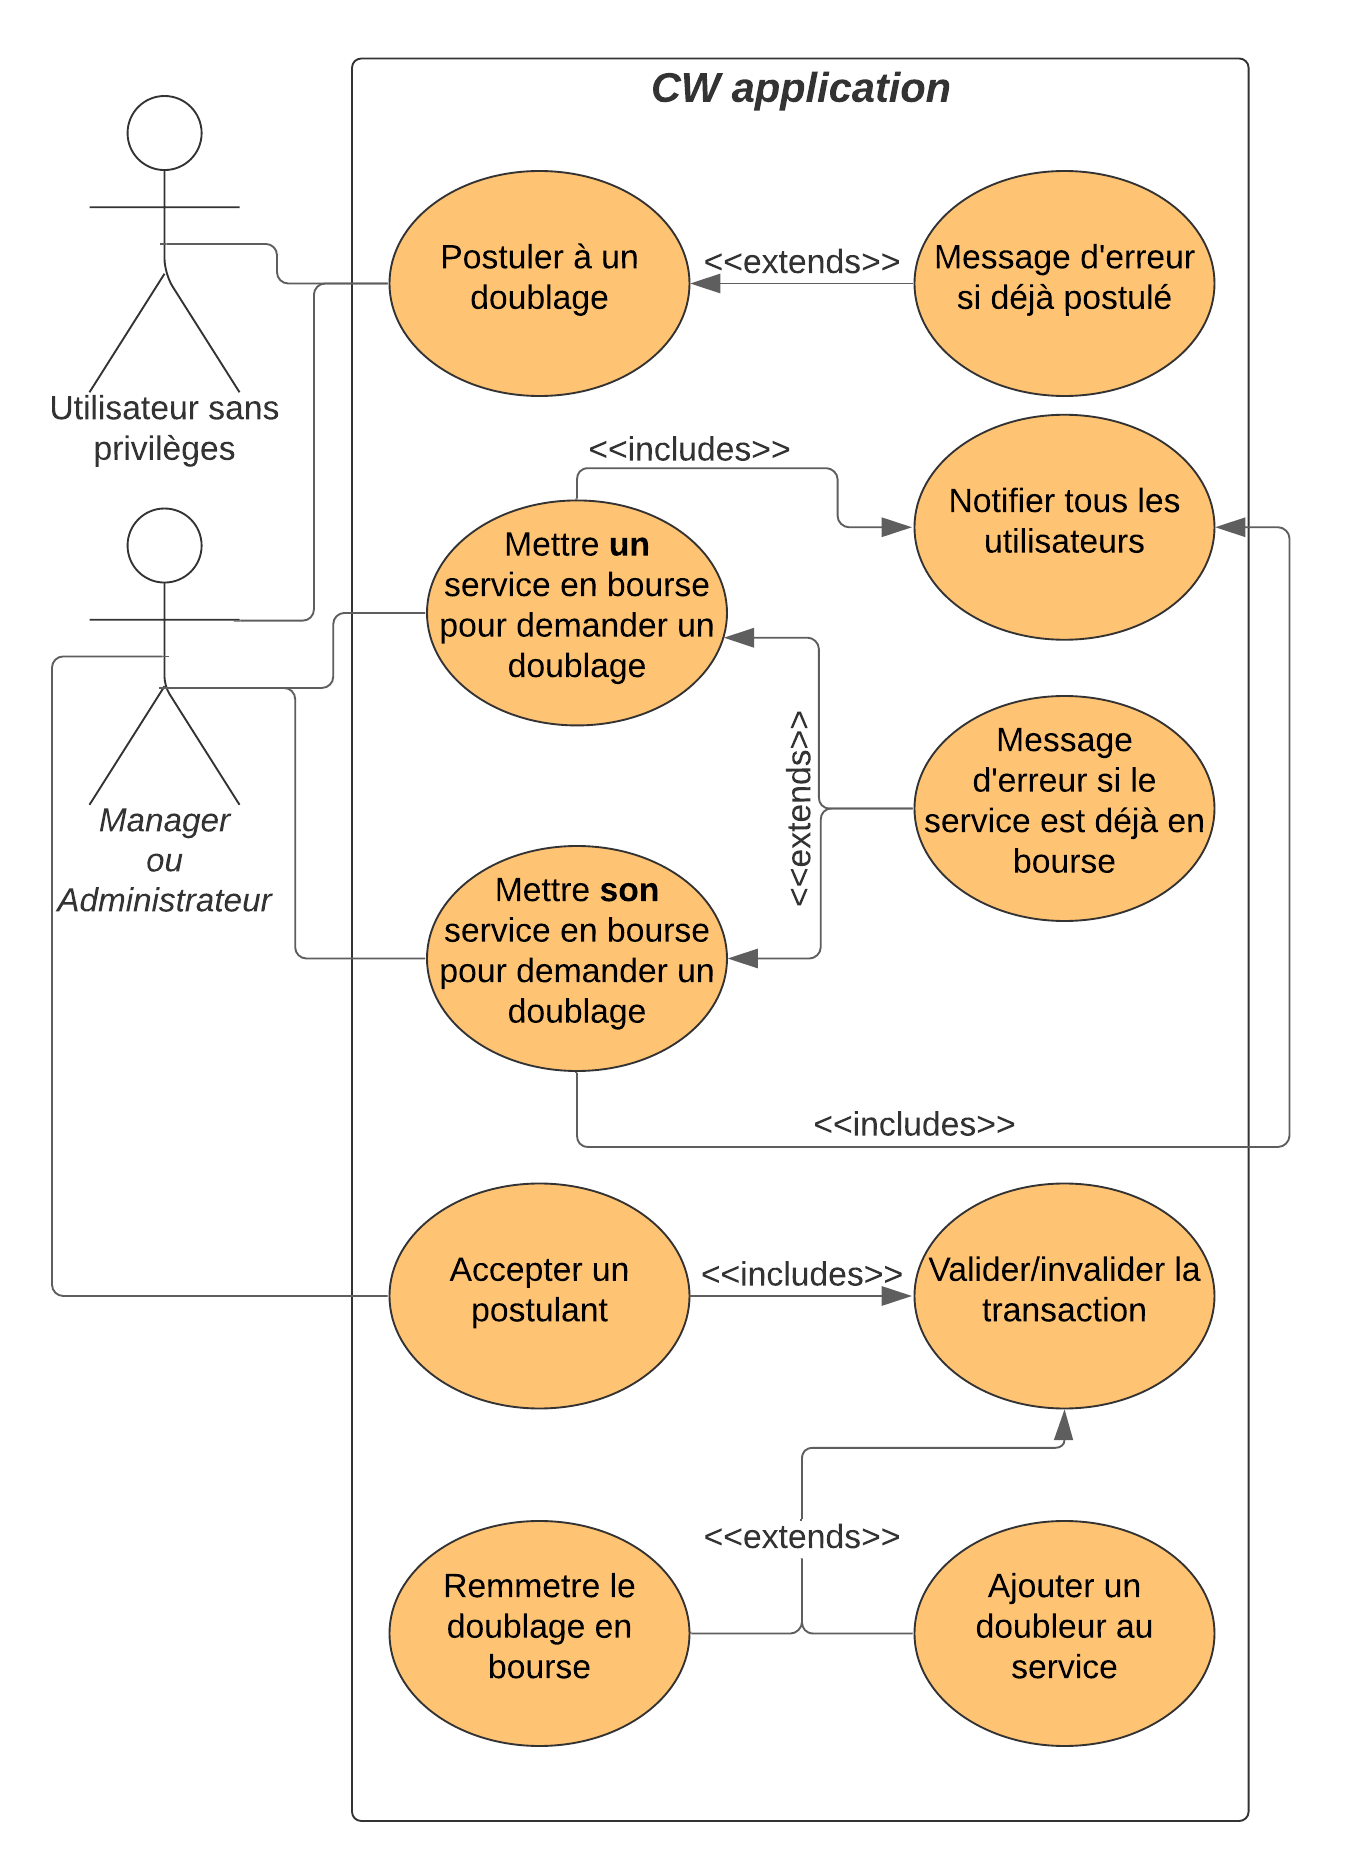
\includegraphics[width= 0.75\textwidth]{uses cases/doublageUC.png}
    \end{center}
    \caption{use case: mise en bourse d'un doublage}
\end{figure}

Les serveur$\cdot$euses sans privilèges ne peuvent que postuler pour des doublages déjà en bourse. Par contre, les utilisateurs avec privilèges peuvent compte à eux faire des demandes de doublage autant pour des services dans lesquels ils ne travaillent pas comme des services dans lesquels ils travaillent. Ils ont aussi la faculté d'accepter des postulants.

\section{Choix des technologies}
Le développement d'applications
pour smartphones est, depuis un peu plus d'une décennie, en pleine effervescence. Il existe, par
conséquent, une multitude de frameworks, services, langages, méthodologies et paradigmes liés à leur
développement.

Ces technologies aux noms exotiques, aux logos plus brillants les uns que les autres et aux
conférences accrocheuses qui leur sont dédiées, font que leurs différences relèvent plus
d'une stratégie marketing visant les informaticiens, réussie que des attributs
intrinsèques de la technologie en question.

Les fonctionnalités de l'application vues précédemment étant d'une complexité modérée et ne demandant pas de ressources importantes
comme tel pourrait être le cas pour une messagerie instantanée à grand échelle ou une application
utilisant abondamment un domaine spécifique de connaissance comme le \textit{machine learning}, le traitement d'images, les jeux vidéo, etc.
Exclu \textit{de facto} le choix d'une technologie basée exclusivement sur les performances ou sur le développement natif.

N'ayant jamais fait cela auparavant, il n'y a aucune préférence de ma part pour telle ou telle technologie.

Ces constats donnent lieu aux critères de sélection suivants:
\smallskip
\begin{itemize}
    \item Développement cross-plateforme
    \item Simplicité
    \item Apprentissage d'un langage plutôt qu'une multitude
    \item Vaste documentation et ressources d'apprentissage
\end{itemize}
\smallskip
Le premier critère est celui qui réduit le plus la liste des possibilités. En effet, les frameworks
permettant le développement d'applications pour Android et IOS ne se comptent pas en grand nombre. Il existe\footnote{Liste non exhaustive}:
\smallskip
\begin{itemize}
    \item Xamarin - Microsoft
    \item React Native - Facebook
    \item Flutter - Google
    \item Adobe PhoneGap - Adobe
    \item Ionic - MIT
\end{itemize}
\smallskip
Le choix parmi ces possibilités découle essentiellement de l'arbitraire. Toutefois, Ionic a été exclu car il est nécessaire de maîtriser HTML5 et par conséquent CSS mais encore Angular JS. Ce qui contredit le 3ème critère.

React native et Xamarin ont été exclus pour des raisons similaires. I.e. l'apprentissage de divers langages.

Finalement, à la suite d’un cours de Academind d'une durée de 40 heures portant sur les aspects les plus basiques du développement jusqu'au déploiement de l'application en passant par le routage, la gestion de requêtes http, la connexion à tout un écosystème de bases de données, l'utilisation de caméra et géolocalisation, et même sur comment changer le logo de l'application, le choix s'est porté sur Flutter.

Flutter est un framework crée par Google. Ce dernier offre, pour les applications, le service Firebase qui englobe :

\smallskip
\begin{itemize}
    \item Cloud Firestore
    \item Real time database
    \item Functions
    \item Machine learning
    \item Cloud messaging
    \item \dots
\end{itemize}
\smallskip
Firebase s'intègre, par conception, particulièrement bien et facilement à Flutter. Même s'ils sont
indépendants, leurs utilisation conjointe forme un seul écosystème plus facile à appréhender. Ainsi pour la
base de données, le choix a été la Real Time Database. Car cette dernière fournit une API REST.

De plus, toujours dans cet écosystème, \textit{Cloud messaging} est utilisé pour l'envoi des notifications et \textit{Functions} pour
effectuer des actions côté serveur lorsque la base de données subit des modifications.
